\chapter{Thermal field theory}

\TODO{add sources of inspiration!!}

\TODO{need to study coherent states for bosons and ferimons???}

\newcommand{\transampl}{\braket{\phi_B | e^{- i \hat{H} T / \hbar} | \phi_A}}

In this chapter, we will develop a theory for studying quantum fields at finite temperature $T$.
We will see that there is an elegant mathematical analogy between the path integral for the transition amplitude of a process and the partition function $Z$ of statistical mechanics, allowing us to express the latter in terms of the former.

In a quantum system in the grand canonical ensemble, the partition function is 
\begin{equation}
	Z = \trace \left( e^{-\beta (\hat{H} - \mu_i \hat{N}_i)} \right) = e^{-\beta \Omega} ,
\label{eq:tft:partition_function}
\end{equation}
where $\hat{H}$ is the Hamiltonian operator $\beta = 1 / k_B T$, $\mu$ is the chemical potential, $\hat{N}_i$ are number operators, $\Omega = -k_B T \log{Z}$ is the grand potential, $k_B$ is the Boltzmann constant and the trace can be evaluated in any basis.
If we can find the partition function, we can obtain all thermodynamic information about the system, such as \cite[chapter 5]{ref:jensoluf}
\begin{align}
	%\text{the entropy}                     \quad \thermalavg{S}   &= -\pdv{\Omega}{T} \\
	           & \text{the average number of particles} & \thermalavg{N_i} & = k_B T \pdv{\log{Z}}{\mu_i},                    & \\
	           & \text{the average energy}              & \thermalavg{E}   & = \mu_i \thermalavg{N_i} - \pdv{\log{Z}}{\beta}  & \\ % \Omega + T S + \mu_i \thermalavg{N_i} \\
	\text{and} & \text{the average pressure}            & \thermalavg{P}   & = \frac{k_B T}{V} \log{Z}.                       &    % -\pdv{\Omega}{V}
\end{align}
This is exactly what we eventually want to insert into the TOV equation \eqref{eq:tov}.
As all relevant information about a system can be derived from the partition function, we say that we have ``solved the system completely'' once we have found $Z$.

First, we will review how the transition amplitude for a process can be expressed as a path integral.
Then we will show how a few adjustments can be made to the path integral in order for it to express the partition function $Z$.
We will show that the path integral expression for the partition function turns out to be the same for bosonic and fermionic fields, although their mathematical fundament is quite different.
Finally, we will consider the specific case of a fermionic gas and find its partition function.

\section{Summary of quantization of quantum fields}

%TODO: should i have a $t$ as in $\ket{\phi(t)}$ ?)

Consider a quantum field theory with Schrödinger-picture field operators $\hat{\phi}(\vec{x})$ and conjugate momenta $\hat{\pi}(\vec{x})$ and Hamiltonian operator
\begin{equation}
	\hat{H} = \int \dif^3 x \, \ham(\hat{\pi}(\vec{x}), \hat{\phi}(\vec{x})) .
\end{equation}
In analogy with position $x$ and momentum $p$ in classical mechanics, we will refer to $\hat\phi(\vec{x})$ and $\hat\pi(\vec{x})$ as operators in ``position-space'' and ``momentum-space''.
%Whether ``position'' refers to $\vec{x}$ or $\phi(\vec{x})$ will therefore depend on context.

The field operators $\hat{\phi}(\vec{x})$ and $\hat{\pi}(\vec{x})$ have eigenstates $\ket{\phi}$ and $\ket{\pi}$ with corresponding eigenvalues $\phi(\vec{x})$ and $\pi(\vec{x})$ at every point $\vec{x}$, as expressed by the eigenvalue equations
\begin{equation}
	\hat{\phi}(\vec{x}) \ket{\phi} = \phi(\vec{x}) \ket{\phi}
	\qquad \text{and} \qquad
	\hat{\pi}(\vec{x}) \ket{\pi} = \pi(\vec{x}) \ket{\pi} .
\label{eq:tft:field_eigenvalue_equations}
\end{equation}

By assumption, the field and the momentum satisfy the commutation relations
\begin{equation}
	\comm{\hat{\phi}(\vec{x})}{\hat{\pi}(\vec{y})} = i \hbar \delta(\vec{x} - \vec{y})
	\qquad \text{and} \qquad
	\comm{\hat{\phi}(\vec{x})}{\hat{\phi}(\vec{y})} = 
	\comm{\hat{\pi}(\vec{x})}{\hat{\pi}(\vec{y)}} = 
	0
\label{eq:tft:boson_field_commutators}
\end{equation}
for bosons, while for fermions they instead satisfy the anticommutation relations
\begin{equation}
	\acomm{\hat{\phi}(\vec{x})}{\hat{\pi}(\vec{y})} = i \hbar \delta(\vec{x} - \vec{y})
	\qquad \text{and} \qquad
	\acomm{\hat{\phi}(\vec{x})}{\hat{\phi}(\vec{y})} = 
	\acomm{\hat{\pi}(\vec{x})}{\hat{\pi}(\vec{y)}} = 
	0 .
\label{eq:tft:fermion_field_anticommutators}
\end{equation}
% peskin eq. 2.20: in Heisenberg picture, these hold at *equal times*

The position-space eigenstates are orthogonal and complete in the sense
\begin{equation}
	\braket{\phi | \phi'} = \prod_{\vec{x}} \delta(\phi(\vec{x}) - \phi'(\vec{x}))
	\qquad \text{and} \qquad
	\int \dif \phi \ket{\phi} \bra{\phi} = 1 .
	\label{eq:tft:orthogonality_completeness_position}
\end{equation}

\newcommand{\posmom}[2]{\exp \left(  \frac{i}{\hbar} \int \dif^3 x \, #2(\vec{x}) #1(\vec{x}) \right)}
\newcommand{\mompos}[2]{\exp \left( -\frac{i}{\hbar} \int \dif^3 x \, #1(\vec{x}) #2(\vec{x}) \right)}
If we find the inner product $\braket{\phi | \pi}$, we can use it together with the completeness relation \eqref{eq:tft:orthogonality_completeness_position} to express position-space states and momentum-space states in terms of each other through
\begin{equation}
	\ket\pi = \int \dif \phi \ket\phi \braket{\phi | \pi} %= \int \dif \phi \posmom{\phi}{\pi}
	\qquad \text{or} \qquad
	\ket\phi = \int \dif \pi \ket\pi \braket{\pi | \phi} . %= \int \dif \phi \mompos{\pi}{\phi} .
\end{equation}
To do so, let us use the position-space representation $\hat{\pi} = (\hbar / i) \fdv{}/{\phi}$ of the momentum operator.
This gives us a first-order differential equation
\begin{equation}
	\braket{\phi | \hat{\pi} | \pi} = \pi(\vec{x}) \braket{\phi | \pi} = \frac{\hbar}{i} \fdv*{\braket{\phi | \pi}}{\phi}
\end{equation}
for the inner product $\braket{\phi | \pi}$.
Choosing the solution with prefactor $1$, we obtain
\begin{equation}
	\braket{\phi | \pi} = \posmom{\phi}{\pi} .
	\label{eq:tft:inner_product_position_momentum}
\end{equation}

The momentum states are also orthogonal and complete, but with slightly different factors.
Due to our convention \eqref{eq:pre:delta_function} for the delta function, orthogonality takes the form
\begin{equation}
\begin{split}
	\braket{\pi_a | \pi_b} &= \int \dif \phi \braket{\pi_a | \phi} \braket{\phi | \pi_b} \\
	                       &= \int \dif \phi \exp \left( i \int \dif^3 x \, (\pi_b(\vec{x}) - \pi_a(\vec{x})) \phi(\vec{x}) / \hbar \right) \\
						   &= 2 \pi \hbar \, \delta(\pi_a(\vec{x}) - \pi_b(\vec{x})) .
\end{split}
\end{equation}
To find the completeness relation, we postulate it up to a constant $B$.
Consider
%Inserting a complete set of both position and momentum states and using the inner product \eqref{eq:tft:inner_product_position_momentum}, consider
\begin{equation}
\begin{split}
	1 &= \int \frac{\dif \pi(\vec{x})}{B} \ket{\pi} \bra{\pi} \\
	  &= \int \frac{\dif \pi(\vec{x})}{B} \ket{\pi} \int \frac{\dif \pi'(\vec{x})}{B} \int \dif \phi(\vec{x}) \braket{\pi | \phi} \braket{\phi | \pi'} \bra{\pi'} \\
	  &= \int \frac{\dif \pi(\vec{x})}{B} \ket{\pi} \int \frac{\dif \pi'(\vec{x})}{B} \underbrace{\int \dif \phi(\vec{x}) \exp \left( \frac{i}{\hbar} \int \dif^3 x \, \left( \pi'(\vec{x}) - \pi(\vec{x}) \right) \phi(\vec{x}) \right)}_{2 \pi \hbar \, \delta(\pi'(\vec{x}) - \pi(\vec{x}))} \bra{\pi'} \\
	  &= \frac{2 \pi \hbar}{B} \underbrace{\int \frac{\dif \pi(\vec{x})}{B} \ket{\pi} \bra{\pi}}_{1} .
\end{split}
\end{equation}
This would be inconsistent unless $B = 2 \pi \hbar$, so completeness in momentum-space is
\begin{equation}
	\int \frac{\dif \pi(\vec{x})}{2 \pi \hbar} \ket{\pi} \bra{\pi} = 1 .
\end{equation}

\section{Path integral for bosonic partition function}

When the Hamiltonian $\hat{H}$ is independent of time, a quantum system evolves from an initial state $\ket{\phi_A}$ to the state $e^{-i \hat{H} T / \hbar} \ket{\phi_A}$ during the time $T$ \cite[equation 2.28]{ref:sakurai}.
Later we will study statistical mechanics for a star in thermal equilibrium -- then the Hamiltonian is always independent of time, otherwise the system would not be in equilibrium.
The transition amplitude for going from the state $\ket{\phi_A}$ to a different state $\ket{\phi_B}$ in the time $T$ is therefore
\begin{equation}
	\transampl \qquad (A \rightarrow B) .
	\label{eq:tft:transition_amplitude_intro}
\end{equation}
Let us demonstrate how this transition amplitude can be written as a path integral.
First, split the time interval $T$ into $N$ intervals $\Delta t = T / N$, and decompose the evolution operator $e^{- i \hat{H} T / \hbar}$ into equally many products of $e^{- i \hat{H} \Delta t / \hbar}$ to write
\newcommand\pointarrow[1]{\underset{\underset{\displaystyle #1}{\displaystyle \uparrow}}{}}
\begin{equation}
	\transampl = \braket{\phi_B | e^{- i \hat{H} \Delta t / \hbar} \cdots e^{- i \hat{H} \Delta t / \hbar} \cdots e^{- i \hat{H} \Delta t / \hbar} | \phi_A} .
\label{eq:tft:time_evolution_splitting}
\end{equation}
%\transampl = \braket{\phi_b | \pointarrow{4} e^{- i H \Delta t} \,\, \cdots \pointarrow{3} e^{- i H \Delta t} \pointarrow{2} \cdots \,\, e^{- i H \Delta t} \pointarrow{1} | \phi_a}
We will take the limit $N \rightarrow \infty$ in the end, so we assume that each interval $\Delta t$ is small.
Now comes the most important trick -- take a deep breath and do the following.
\begin{itemize}
\item Insert $N$ complete sets of \emph{momentum} states $1 = \int \dif \pi_n / (2 \pi \hbar) \ket{\pi_n} \bra{\pi_n}$ to the \emph{left} of every exponential, including the rightmost one, with $n$ increasing from right to left.
\item Insert $N-1$ complete sets of \emph{position} states $1 = \int \dif \phi_n \ket{\phi_n} \bra{\phi_n}$ to the \emph{right} of every exponential, excluding the rightmost one, with $n$ increasing from right to left.
\end{itemize}
Now exhale.
With this trick, the transition amplitude can be written as the product
\begin{equation}
	\transampl = \prod_{n=0}^{N} \int \frac{\dif \phi_n \dif \pi_n}{2 \pi \hbar} 
	             \braket{\phi_{n+1} | \pi_n} \braket{\pi_n | e^{- i \hat{H} \Delta t / \hbar} | \phi_n} ,
\label{eq:tft:transition_amplitude_product}
\end{equation}
where we have defined $\ket{\phi_0} = \ket{\phi_A}$ and $\ket{\phi_{N+1}} = \ket{\phi_B}$.
The inner products $\braket{\phi_{n+1} | \pi_n}$ can simply be replaced by the exponential \eqref{eq:tft:inner_product_position_momentum}, so let us turn our attention to the matrix elements $\braket{\pi_n | e^{- i \hat{H} \Delta t / \hbar} | \phi_n}$.
Since the time step $\Delta t$ is assumed small, we can expand the exponential $e^{- i \hat{H} \Delta t / \hbar} \taylor 1 - i \hat{H} \Delta t / \hbar$ to first order in time.
Under the assumption that the Hamiltonian $\hat{H}$ is a sum of terms with all \emph{position}-space operators $\hat{\phi}$ on the \emph{right} and all \emph{momentum}-space operators $\hat{\pi}$ on the \emph{left}, we can pull it out of the product at the additional benefit of replacing its operators by their eigenvalues.
We then obtain
\begin{equation}
\begin{split}
	\braket{\pi_n | e^{- i \hat{H} \Delta t / \hbar} | \phi_n} &\taylor \braket{\pi_n | (1 - i \hat{H} \Delta t / \hbar) | \phi_n} \\
	                                                   &=       \braket{\pi_n | \phi_n} (1 - i H_n \Delta t / \hbar) \\
	                                                   &\taylor \braket{\pi_n | \phi_n} e^{- i H_n \Delta t / \hbar}, \\
\end{split}
\label{eq:tft:path_integral_hamiltonian_assumption}
\end{equation}
where we no longer have any operators, but only the Hamiltonian eigenvalue at the $n$-th timestep
\begin{equation}
	H_n = \int \dif^3 x \, \ham(\pi_n(\vec{x}), \phi_n(\vec{x})) .
\label{eq:tft:hamiltonian_eigenvalues}
\end{equation}
Note the importance of expanding the exponential to first order in timeonly.
If the Hamiltonian contained \emph{any} mixed sequence of operators such as $H \propto \hat{\pi} \hat{\phi}$, then higher powers like $\hat{H}^2 \propto \hat{\pi} \hat{\phi} \hat{\pi} \hat{\phi}$ in the power series expansion of the time evolution operator would not be in the assumed left-right order.

\TODO{spør Jens Oluf om et alternativt argument her -- kan ikke bare operatorer i $\hat{H}$ kommuteres inntil man får den ønskede rekkefølgen, samtidig som ekstra konstanter medfører en fysisk ubetydelig fase? F.eks. $\hat{H} = \hat{p} \hat{q} = \hat{q} \hat{p} \pm i \hbar$, men de to har forskjellige egenverdier $pq$ og $pq \pm i \hbar$??? Men dette er alltid en fysisk ubetydelig fase?}

\iffalse
(TODO: If the Hamiltonian is \emph{not} in the order we assumed above, we could always bring it into this order by commuting operators using the commutation relation \eqref{eq:tft:boson_field_commutators}.
But such terms would appear only as a constant phase on the right side of \eqref{eq:tft:path_integral_hamiltonian_assumption} that would not depend on the dynamics of the process.
AHence, we can relax this assumption by absorbing this physically irrelevant phase into the transition amplitude. ER DETTE RIKTIG? INGEN LÆREBØKER NEVNER DETTE.)

(TODO: if this argument holds, then it can be applied for any $\hat{H}^n$, and there is no reason to expand to first order in time, either)
\fi

\begin{figure}
\centering
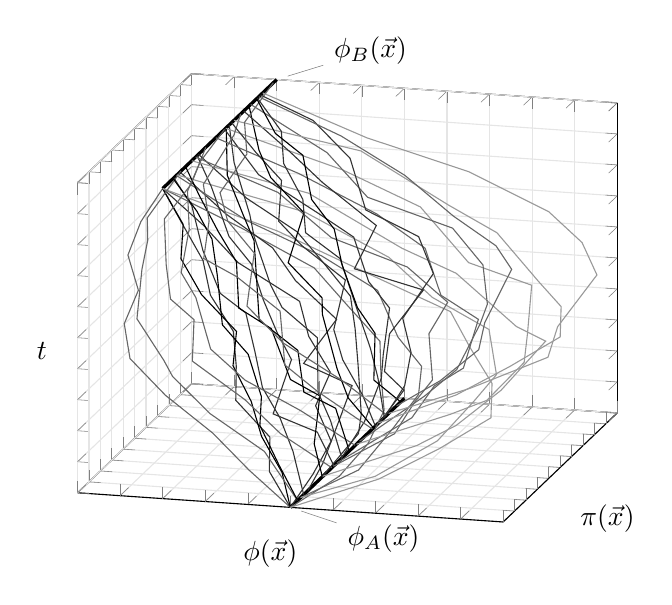
\begin{tikzpicture}
\begin{axis}[
	clip=false,
	view={-75}{20}, 
	%xtick=\empty, ytick=\empty, ztick=\empty, 
	xticklabel=\empty, yticklabel=\empty, zticklabel=\empty,
	xlabel=$\pi(\vec{x})$, ylabel=$\phi(\vec{x})$, zlabel=$t$, zlabel style={rotate=-90},
	%x label style={at={(axis description cs:0.5,0.0)},anchor=north},
	%y label style={at={(axis description cs:0.5,0.0)},anchor=north},
	%z label style={at={(axis description cs:0.5,0.0)},anchor=north},
	xmin=0, xmax=1, ymin=0, ymax=1, zmin=0, zmax=5,
	xtick distance=0.1, ytick distance=0.1, ztick distance=0.5, grid=major, grid style={solid, thin, black!10!white},
	%extra x ticks={0j
	declare function={
		phi1 = 0.5;
		phi2 = 0.8;
		randbetween(\a,\b) = \a + (\b - \a) / 2 * rand;
		%randradius(\x, \rmin, \rmax) = randbetween(\rmin, \rmax) * (\x-0) * (\x-1);
		randfunc(\x,\rmin,\rmax) = randbetween(\rmin,\rmax) * (\x-0)*(\x-1) * 4; % and(x>=0.01, x<=0.99); %(\x-0) * (\x-1);
	},
]
\addplot3 [domain=0:1, samples=2, very thick] ({x}, {phi1}, {0}) node [pos=0.0,pin={-8:$\phi_A(\vec{x})$}] {};
\addplot3 [domain=0:1, samples=2, very thick] ({x}, {phi2}, {5}) node [pos=1.0,pin={+5:$\phi_B(\vec{x})$}] {};
\pgfplotsinvokeforeach{0.0, 0.2, ..., 1.0} {
	\addplot3 [domain=0:1, samples=10, domain y=0:1, samples y=1, black!60!white]  ({max(0, min(1, #1+randbetween(-0.1,0.1))}, {phi1 + (phi2-phi1)*x + randfunc(x,-0.2,-0.3)}, {5*x});
	\addplot3 [domain=0:1, samples=10, domain y=0:1, samples y=1, black!80!white]  ({max(0, min(1, #1+randbetween(-0.1,0.1))}, {phi1 + (phi2-phi1)*x + randfunc(x,-0.0,-0.1)}, {5*x});
	\addplot3 [domain=0:1, samples=10, domain y=0:1, samples y=1, black!100!white] ({max(0, min(1, #1+randbetween(-0.1,0.1))}, {phi1 + (phi2-phi1)*x + randfunc(x,+0.0,+0.1)}, {5*x});
	\addplot3 [domain=0:1, samples=10, domain y=0:1, samples y=1, black!80!white]  ({max(0, min(1, #1+randbetween(-0.1,0.1))}, {phi1 + (phi2-phi1)*x + randfunc(x,+0.2,+0.3)}, {5*x});
	\addplot3 [domain=0:1, samples=10, domain y=0:1, samples y=1, black!60!white]  ({max(0, min(1, #1+randbetween(-0.1,0.1))}, {phi1 + (phi2-phi1)*x + randfunc(x,+0.4,+0.5)}, {5*x});
	\addplot3 [domain=0:1, samples=10, domain y=0:1, samples y=1, black!40!white]  ({max(0, min(1, #1+randbetween(-0.1,0.1))}, {phi1 + (phi2-phi1)*x + randfunc(x,+0.6,+0.7)}, {5*x});
	%\addplot3 [domain=0:1, samples=10, domain y=0:1, samples y=1] ({#1+randfunc(x,0.2,0.3)}, {phi1 + (phi2-phi1)*x + randfunc(x,0.1,0.2)}, {5*x});
}
\end{axis}
\end{tikzpicture}
\caption{\label{fig:phase_space}A quantum system that evolves from the initial field $\phi_A(\vec{x})$ to the final field $\phi_B(\vec{x})$ can take all possible paths through phase space, but some are more likely than others. The conjugate momentum field $\pi(\vec{x})$ does not need to be the same at the start and the end.}
\end{figure}

Substituting \cref{eq:tft:inner_product_position_momentum,eq:tft:path_integral_hamiltonian_assumption,eq:tft:hamiltonian_eigenvalues}, the transition amplitude \eqref{eq:tft:transition_amplitude_product} becomes
\begin{equation}
\begin{split}
	\transampl &=      \left( \prod_{n=1}^N \int \frac{\dif \phi_n \dif \pi_n}{2 \pi \hbar} \right) \\
	           &\times \exp \left( \frac{i \Delta t}{\hbar} \sum_{n=1}^N \int \dif^3 x \left( \pi_n(\vec{x}) \frac{\phi_{n+1}(\vec{x}) - \phi_n(\vec{x})}{\Delta t} - \ham(\pi_n(\vec{x}), \phi_n(\vec{x})) \right)
	\right)
\end{split}
\end{equation}
Finally, we take the continuum limit by sending $N \rightarrow \infty$.
It is then natural to define
$\phi(\vec{x}, t_n) = \phi_n(\vec{x}, t_n)$
and
$\pi(\vec{x}, t_n) = \pi_n(\vec{x}, t_n)$
to be the values of the fields at each timestep $t_n$.
Both become continuous functions of time in the continuum limit.
We also use the finite difference definition of the derivative to turn the fraction in the exponential into a partial derivative $\dot{\phi}(\vec{x},t) = \pdv{\phi(\vec{x},t)}/{t}$.
Similarly, we use the Riemann sum definition of the integral to turn the sum $\sum \Delta t$ into an integral $\int \dif t$.
We also define the \textbf{functional integrals}
\begin{equation}
	\int \pathintdif \phi = \lim_{N \rightarrow \infty} \prod_{n=1}^{N} \int \dif \phi_n
	\qquad \text{and} \qquad
	\int \pathintdif \pi = \lim_{N \rightarrow \infty} \prod_{n=1}^{N} \int \frac{\dif \pi_n}{2 \pi \hbar} .
\label{eq:tft:functional_integral}
\end{equation}
%We have swept the diverging factor $(2 \pi \hbar)^N$ under the rug, arguing that it contains no physical information about the dynamics of the process and can be ignored, unlike the other factors.
%TODO: can integrate out momentum with gaussian integral if it appears as $p^2$)
With all of these steps, the transition amplitude takes the form of the \textbf{path integral}
\begin{equation}
\begin{split}
	\transampl &=      \int \pathintdif \pi \int_{\phi(\vec{x}, 0)=\phi_A(\vec{x})}^{\phi(\vec{x},T)=\phi_B(\vec{x})} \pathintdif \phi \\
	           &\times \exp \left( \frac{i}{\hbar} \int_0^T \dif t \int \dif^3 x \left( \pi(\vec{x}, t) \dot{\phi}(\vec{x}, t) - \ham(\pi(\vec{x}, t), \phi(\vec{x}, t)) \right) \right) .
\end{split}
\label{eq:tft:path_integral_hamiltonian}
\end{equation}

It is tempting to recognize $\pi \dot\phi - \ham$ as the Legendre transformation that converts to the Lagrangian density and write $\lagr$ in its place.
But we should be careful -- the Legendre transformation converts the independent variable $\dot\phi$ in $\lagr(\phi, \dot\phi, \nabla\phi)$ to $\pi$ in $\ham(\phi, \pi, \nabla\phi)$.
We are integrating over $\pi$ and should therefore not lose track of it by writing $\lagr = \lagr(\phi, \dot\phi, \nabla\phi)$.
Thus, we do not modify the integral further.
\TODO{does this make sense?}

\TODO{write just $\ham$ etc. instead to make notation lighter, then write in text the arguments?}

\iffalse
Note that the combination of the Hamiltonian and the fields in the exponential is precisely the Legendre transformation that converts between the Hamiltonian density $\ham$ and the Lagrangian density $\lagr$.
Thus, we might as well express the transition amplitude as the \textbf{path integral}
%	\transampl = \int \pathintdif \pi \int_{\phi_A(\vec{x}, 0)}^{\phi_B(\vec{x}, T)} \pathintdif \phi \\
%	             \exp \left( i \int_0^T \dif t \int \dif^3 x \, \left( \lagr(\pi(\vec{x}, t), \phi(\vec{x}, t)) \right) \right) .
\begin{equation}
	\transampl = \int \pathintdif \pi \int_{\phi_A(\vec{x})}^{\phi_B(\vec{x})} \pathintdif \phi \, \exp \big( i S \left[ \pi(\vec{x}, t), \phi(\vec{x}, t) \right] / \hbar \big) ,
\label{eq:tft:path_integral_lagrangian}
\end{equation}
with the action
\begin{equation}
	S \left[ \pi(\vec{x}, t), \phi(\vec{x}, t) \right] = \int_0^T \dif t \int \dif^3 x \, \lagr \left( \pi(\vec{x}, t), \phi(\vec{x}, t) \right) . \qquad \text{TODO: factor $c$?}
\label{eq:tft:action}
\end{equation}
\fi
The path integral expresses the transition amplitude for the process $A \rightarrow B$ as a sum over all possible paths through phase space, each weighted by the value on the unit circle with phase corresponding to the action of the path.
This interpretation is illustrated in \cref{fig:phase_space}.
Note that the position-space integral $\int \pathintdif \phi$ is constrained to start and end in the initial and final states, but the momentum integral $\int \pathintdif \pi$ has no such constraint.

Why have we spent so much time on this transition amplitude, when we really are only interested in the partition function \eqref{eq:tft:partition_function}?
If we evaluate the trace \eqref{eq:tft:partition_function} in the basis of fields $\ket{\phi_0}$, we obtain
\begin{equation}
	Z = \int \dif \phi_0 \braket{\phi_0 | e^{-\beta (\hat{H} - \mu_i \hat{N}_i)} | \phi_0} .
\end{equation}
This is precisely an integral over transition amplitudes \eqref{eq:tft:path_integral_hamiltonian}, but now with 
\begin{itemize}
\item equal start and end states $\ket{\phi_A} = \ket{\phi_B} = \ket{\phi_0}$, 
\item the Hamiltonian $\hat{H} - \mu_i \hat{N}_i$ and 
\item a purely imaginary time variable $t = -i \tau$ with $\tau$ running from $0$ to $\beta \hbar$.
\end{itemize}
The change from a real to imaginary time variable can be accomplished by a Wick rotation that does not change the value of the integral \TODO{true?}.
Thus, we can express the partition function as path integrals \eqref{eq:tft:path_integral_hamiltonian} with these substitutions!
This yields
\begin{equation}
	Z = \int \pathintdif \pi \oint_+ \pathintdif \phi \, \exp \left( \frac{1}{\hbar} \int_0^{\beta \hbar} \dif \tau \int \dif^3 x \left( i \pi \dot{\phi} - \ham + \mu \numdensity) \right) \right)
\label{eq:tft:bosonic_partition_function}
\end{equation}
where we have absorbed $\int \dif \phi_0$ into the path integral $\int \pathintdif \phi$ and write $\oint_+$ to indicate that we integrate over all fields $\phi(x, \tau) = \phi(x, \tau + \beta \hbar)$ that are \emph{periodic} in ``imaginary time'' $\tau$, due to the equal start and end states $\phi_A(\vec{x}) = \phi_B(\vec{x})$ in \cref{eq:tft:path_integral_hamiltonian}.
Thus, thermal field theory -- statistical mechanics for quantum fields at finite temperature -- is essentially equivalent to ordinary quantum field theory with temperature-dependent time and periodic fields, and the partition function is obtained by integrating along closed paths in phase space!

We have not yet discussed the appearance of the chemical potential $\mu$ and the number density $\numdensity$ in the path integral.
If the theory admits one or more conserved conserved currents $j_i^\mu$ with $\partial_\mu j_i^\mu$ by Noether's theorem, there are associated conserved charges $Q_i = \int \dif^3 x \, j_i^0$.
For every such conserved charge, we can associate a chemical potential $\mu_i$ and include the term
\begin{equation}
	\mu_i \numdensity_i = \mu_i j_i^0
\label{eq:tft:chemical_potential}
\end{equation}
in the path integral.
For example, if the theory has particles and antiparticles, then a conserved charge typically corresponds to the difference between the number of particles and antiparticles in the system.
The chemical potential can then be interpreted as a knob with which we can regulate the balance between particles and antiparticles in the system.
We will later see examples of theories both with and without conserved charges.

\TODO{i do not understand properly how the chemical potential works and why we can include it}

\section{Path integral for fermionic partition function}

%(TODO: see random_note_1.pdf)

For fermions, commutators are replaced by anticommutators, and so eigenvalues no longer commute, but anticommute!
To obtain the path integral formulation of the fermionic partition function, we must therefore use anticommuting \textbf{Grassmann numbers} instead of commuting complex numbers.

For concreteness, consider fermions described by the Dirac Lagrangian
\begin{equation}
	\lagr = \bar{\psi} (i \hbar c \slashed\partial - m c^2) \psi .
\end{equation}
Here, the conjugate momentum turns out to be
\begin{equation}
	\pi = \fdv{\lagr}{\dot\psi} = i \hbar \psi^\dagger ,
\label{eq:tft:dirac_conjugate_momentum}
\end{equation}
so, perhaps confusingly, we are instructed to treat the field and its conjugate as independent variables in the path integral.

To evaluate the bosonic partition function, we inserted completeness relations for both the field and the conjugate momentum, and we took the trace by integration over fields.
For fermionic fields and Grassmann numbers, these properties are different.

\TODO{show/refer all these, appendix on Grassmann numbers / coherent fermion states?}
First, the inner product between two states is
\begin{equation}
	\braket{\eta_1 | \eta_2} = \exp \left\{ \int \dif^3 x \, \eta_1^\dagger(\vec{x}) \eta_2(\vec{x}) \right\} .
\label{eq:tft:grassmann_inner_product}
\end{equation}
Second, the trace is
\begin{equation}
	\int \dif \eta^\dagger \int \dif \eta \, e^{-\eta^\dagger \eta} \braket{-\eta | A | \eta} = \trace{A} .
\label{eq:tft:trace_grassmann}
\end{equation}
Third, completeness takes the form
\begin{equation}
	\int \dif \eta^\dagger \int \dif \eta \, \exp \left\{-\int \dif^3 x \, \eta^\dagger(\vec{x}) \eta(\vec{x}) \right\} \ket{\eta} \bra{\eta} = 1 .
\label{eq:tft:completeness_grassmann}
\end{equation}

The partition function \eqref{eq:tft:partition_function} follows from the trace \eqref{eq:tft:trace_grassmann} with $A = e^{-\beta (\hat{H} - \mu \hat{N})}$ as
\begin{equation}
	Z = \int \dif \psi_0^\dagger \int \dif \psi_0 \, e^{-\int \dif^3 x \, \psi_{0}^\dagger(\vec{x}) \psi_{0}(\vec{x})} \braket{-\psi_0 | e^{-\beta(\hat{H} - \mu \hat{N})} | \psi_0} .
\end{equation}
Breaking up the operator $e^{\ldots}$ as in \cref{eq:tft:time_evolution_splitting} and inserting one Grassmann completeness relation \eqref{eq:tft:completeness_grassmann} between every factor, the partition function becomes
\begin{equation}
	Z = \prod_n \int \dif \psi_n^\dagger \int \dif \psi_n \, e^{-\int \dif^3 x \, \psi_{n}^\dagger(\vec{x}) \psi_{n}(\vec{x})} \braket{\psi_{n+1} | e^{-(\hat{H} - \mu \hat{N}) \Delta \tau / \hbar} | \psi_n} ,
\end{equation}
where we define $\bra{\psi_{N+1}} = \bra{-\psi_0}$ -- \emph{note the minus sign!}
Next, expand the Hamiltonian to first order as in \cref{eq:tft:path_integral_hamiltonian_assumption}.
Then we obtain
\begin{equation}
	Z = \prod_n \int \dif \psi_n^\dagger \int \dif \psi_n \, e^{-\int \dif^3 x \, \psi_{n}^\dagger(\vec{x}) \psi_{n}(\vec{x})} \braket{\psi_{n+1} | \psi_n} e^{-(H_n - \mu N) \Delta \tau / \hbar} .
\end{equation}
Now use the Grassmann inner product \eqref{eq:tft:grassmann_inner_product} to write
\begin{equation}
	Z = \prod_n \int \dif \psi_n^\dagger \int \dif \psi_n \, \exp \left\{ \frac{\Delta \tau}{\hbar} \sum_n \int \dif^3 x \left( \hbar \frac{\psi^\dagger_{n+1} - \psi^\dagger_n}{\Delta \tau} \psi_{n} - \ham + \mu \numdensity \right) \right\} .
\end{equation}
Finally, take the continuum limit and integrate $\int \dif \tau \, \dot{\psi^\dagger} \psi = -\int \dif \tau \, \psi^\dagger \dot{\psi}$ by parts \TODO{why is this valid for Grassmann numbers?}.
As in \eqref{eq:tft:functional_integral}, introduce the functional integrals $\pathintdif \psi = \lim_{N \rightarrow \infty} \prod_n \dif \psi_n$ and $\pathintdif [i \hbar \psi^\dagger] = \lim_{N \rightarrow \infty} \prod_n \psi^\dagger$, where we absorb some physically irrelevant prefactors into the latter to preserve similarity between the conjugate momentum $\pi$ and $i \hbar \psi^\dagger$. 
We then obtain the \textbf{fermionic partition function}
\begin{equation}
	Z = \oint_- \pathintdif [i \hbar \psi^\dagger] \oint_- \pathintdif \psi \exp \left\{ \frac{1}{\hbar} \int_0^{\beta \hbar} \dif \tau \int \dif^3 x \left( -\hbar \psi^\dagger \dot{\psi} - \ham ( \psi^\dagger, \psi ) + \mu \numdensity \right) \right\} ,
\label{eq:tft:fermion_partition_function}
\end{equation}
where $\oint_-$ means to integrate over \emph{antiperiodic} fields $\psi(\vec{x}, 0) = -\psi(\vec{x}, \beta \hbar)$, naturally extending the symbol $\oint_+$ we introduced for bosonic fields that were \emph{periodic}.
Apart from the difference in periodicity, this result is -- remarkably -- exactly the same as the bosonic partition function \eqref{eq:tft:bosonic_partition_function}, with canonical momentum \eqref{eq:tft:dirac_conjugate_momentum}!
But the similarity in facade were achieved by a drastically different mathematical fundament.

\TODO{do for general $\psi \rightarrow \eta$ as in random note 1 on the web, then specialize later to Dirac?}

\iffalse
The partition function is therefore
\begin{equation}
\begin{split}
	Z &= \int \dif \psi_0^\dagger \int \dif \psi_0 \, e^{-\psi_{n+1}^\dagger \psi_{n+1}} \braket{-\psi_0 | e^{-\beta(\hat{H} - \mu \hat{N})} | \psi_0} \\
	  &= \prod_n \int \dif \psi_n^\dagger \int \dif \psi_n \, e^{-\psi_{n+1}^\dagger \psi_{n+1}} \braket{\psi_{n+1} | e^{-(\hat{H} - \mu \hat{N}) \Delta \tau / \hbar} | \psi_n} \\
	  &= \prod_n \int \dif \psi_n^\dagger \int \dif \psi_n \, e^{-\psi_{n+1}^\dagger \psi_{n+1}} \braket{\psi_{n+1} | \psi_n} e^{-(H_n - \mu N) \Delta \tau / \hbar} \\
	  &= \prod_n \int \dif \psi_n^\dagger \int \dif \psi_n \, \exp \left\{ -\frac{\Delta t}{\hbar} \sum_n \int \dif^3 x \left( \psi^\dagger_{n+1} \frac{\psi_{n+1} - \psi_n}{\Delta t} + \ham - \mu \numdensity \right) \right\} \\
	  &= \oint_- \pathintdif \psi^\dagger \oint_- \pathintdif \psi \exp \left\{ \frac{1}{\hbar} \int_0^{\beta \hbar} \dif \tau \int \dif^3 x \left( -\psi^\dagger(\vec{x},\tau) \dot{\psi}(\vec{x},\tau) - \ham \left( \psi^\dagger(\vec{x},\tau), \psi(\vec{x},\tau) \right) + \mu \numdensity \right) \right\} \\
\end{split}
\end{equation}
\fi

\section{Matsubara frequencies}

We have just witnessed how the partition function for bosons can be expressed by the path integral \eqref{eq:tft:bosonic_partition_function} with fields that are periodic in imaginary time.
For Dirac fermions, we have showed that we can ``naively'' use the same result by substituting the canonical momentum $\pi = i \hbar \psi^\dagger$ and integrate over antiperiodic fields.
In summary, the field $\psi(\vec{x}, \tau)$ -- here regarded as \emph{either} a bosonic or fermionic field -- satisfies the (anti)periodicity
\begin{equation}
	\phi(\vec{x}, \tau) = \begin{cases}
						      + \phi(\vec{x}, \tau + \beta \hbar) & \text{for bosons} \\
						      - \phi(\vec{x}, \tau + \beta \hbar) & \text{for fermions} .
	                      \end{cases}
\label{eq:tft:periodicity}
\end{equation}
Accordingly, we can expand either field in a Fourier series
\begin{equation}
	\psi(x, \tau) = \sum_n \psi_n(x) e^{i \omega_n \tau}
\end{equation}
with \textbf{Matsubara frequencies} 
\begin{equation}
	\omega_n = \begin{cases}
			       2 \pi n / \beta \hbar    & \text{for bosons} \\
				   2 \pi (n+\frac12) / \beta \hbar & \text{for fermions} .
	           \end{cases}
\label{eq:tft:matsubara_frequencies}
\end{equation}
The offset $+\pi / \beta \hbar$ makes the fermionic field antiperiodic at $\tau = \beta \hbar$.

Although the field is not periodic in space, we can still represent it by its Fourier transform as
\begin{equation}
	\psi_n(x) = \int \frac{\dif^3 k}{(2 \pi / L)^3} \, \psi_n(\vec{k}) e^{i \vec{k} \cdot \vec{x}},
\label{eq:tft:mathematical_fourier_expansion}
\end{equation}
where $L \rightarrow \infty$ is the ``periodicity'' of the field along either axis that is sent to infinity in the Fourier transform, and $V = L^3 \rightarrow \infty$ the corresponding volume.
It will be important to have a ficticious finite volume to work with when we want to convert ``extensive'' observables like the energy $\thermalavg{E}$ into ``intensive'' observables like the energy \emph{density} $\epsilon = \thermalavg{E} / V$ in preparation for using the TOV equation \eqref{eq:tov}.

Ultimately, then, we can expand
\begin{equation}
	\psi(x, \tau) = \sum_n \sum_\vec{k} \psi_n(\vec{k}) e^{i (\vec{k} \cdot \vec{x} + \omega_n \tau)}
\label{eq:tft:fourier_series}
\end{equation}
with the Matsubara frequencies \eqref{eq:tft:matsubara_frequencies}.
To be more compatible with the notation that will follow, we write
\begin{equation}
	V \int \frac{\dif^3 k}{(2 \pi)^3} = \sum_\vec{k}
\label{eq:tft:continuous_limit}
\end{equation}
with a normal summation sign, but really mean the integral in \eqref{eq:tft:mathematical_fourier_expansion}.

The wave number $\vec{k}$ and the Matsubara frequency $\omega_n$ here arose due to geometrical considerations of the periodicity of the field.
Later on, we will see that they have important physical consequences.
In anticipation of this, we define the corresponding momentum and Matsubara energy
\begin{equation}
	\vec{p} = \hbar \vec{k}, \qquad
	E_n = \hbar \omega_n \qquad \text{and} \qquad
	\sum_\vec{p} = \sum_\vec{k} = V \int \frac{\dif^3 p}{(2 \pi \hbar)^3}.
\label{eq:tft:matsubara_energies}
\end{equation}

\section{Partition function for non-interacting bosonic real scalar field}

\TODO{do Bose-Einstein with complex scalar field instead of real scalar field for more ``symmetry'' to the fermionic case?}

As a first example, we apply the path integral formalism to find the partition function for a non-interacting real scalar field representing spin-$0$ bosons.
Its Lagrangian density is
% note: unit of phi is sqrt(energy / length)
\begin{equation}
	\lagr = \frac{1}{2} (\partial_\mu \phi) (\partial^\mu \phi) - \frac12 \frac{m^2 c^2}{\hbar^2} \, \phi^2
	      = \frac{1}{2 c^2} \dot{\phi}^2 - \frac12 (\nabla \phi)^2  - \frac12 \frac{m^2 c^2}{\hbar^2} \, \phi^2 .
\label{eq:tft:boson_lagrangian}
\end{equation}
The conjugate momentum \TODO{ref some general formula?} is
\begin{equation}
	\pi = \pdv{\lagr}{\dot{\phi}} = \frac{1}{c^2} \dot{\phi} .
\end{equation}
The Hamiltonian density is therefore
\begin{equation}
	\ham = \pi \dot{\phi} - \lagr = \frac12 c^2 \pi^2 + \frac12 (\nabla \phi)^2 + \frac12 \frac{m^2 c^2}{\hbar^2} \phi^2 .
\label{eq:tft:boson_hamiltonian}
\end{equation}
We now calculate the partition function \eqref{eq:tft:bosonic_partition_function}.
To do so, we need the combination
\begin{equation}
\begin{split}
	i \pi \dot\phi - \ham &= i \pi \dot\phi - \frac{1}{2} c^2 \pi^2 - \frac12 (\nabla \phi)^2 - \frac{1}{2} \frac{m^2 c^2}{\hbar^2} \phi^2 \\
	                      &= -\frac{1}{2} c^2 \left( \pi - \frac{i}{c^2} \dot\phi \right)^2 - \frac{1}{2 c^2} \dot\phi^2 - \frac{1}{2} (\nabla \phi)^2 - \frac{1}{2} \frac{m^2 c^2}{\hbar^2} \phi^2 \\
	                      &= -\frac{1}{2} c^2 \tilde\pi^2 + \lagr_E . \\
\end{split}
\label{eq:tft:boson_field_combination}
\end{equation}
We completed the square by defining the shifted field $\tilde\pi = \pi - i \dot\phi / c^2$, for reasons that soon will be apparent.
Remember that the Legendre transformation \eqref{eq:tft:boson_hamiltonian} exchanges the independent variable $\dot\phi$ in $\lagr = \lagr(\phi, \dot\phi, \nabla\phi)$ to $\pi$ in $\ham = \ham(\phi, \pi, \nabla\phi)$.
Thus, the shift can be regarded as a shift by a \emph{constant}.
We also defined the remaining terms as the Lagrangian density $\lagr_E$.
It is exactly the original Lagrangian density \eqref{eq:tft:boson_lagrangian}, only with $\tau \rightarrow i \tau$.
This can be interpreted as a change from Minkowski space to Euclidean space, and we therefore call $\lagr_E(\tau) = \lagr(i \tau)$ the Euclidean Lagrangian density.
The path integral \eqref{eq:tft:bosonic_partition_function} is then
\begin{equation}
	Z = \int \pathintdif \pi \oint_+ \pathintdif \phi \exp \left\{ \frac{1}{\hbar} \int_0^{\beta \hbar} \dif \tau \int \dif^3 x \left[ - \frac12 c^2 \tilde\pi^2 + \lagr_E \right] \right\} .
\end{equation}
Since $\tilde\pi$ can be regarded as a constant shift of the field $\pi$, we can now exploit that $\int \pathintdif \tilde\pi = \int \pathintdif \pi$ and then \emph{integrate out} the momentum using the Gaussian integral $\int_{-\infty}^{+\infty} \dif x \, e^{-x^2} = \sqrt{\pi}$ with a suitable rescaling of $x$ (where $\pi \approx 3.1415$, of course -- not the conjugate momentum).
We do not bother keeping track of this constant or any other constants in front of the partition function, as the physical quantities only contain derivatives of the logarithm of $Z$ 

\TODO{ref. integral?}

\TODO{but the pressure contains $\log Z$, not a derivative, so we should not drop terms! is the resolution that, in the end, assuming all ``ghosted terms'' are infinites, we can fix it by cherry picking the non-divergent term for the pressure?}

Thus it only remains to tackle the $\phi$-integral
\begin{equation}
	Z = \oint_+ \pathintdif \phi \exp \left\{ \frac{S_E}{\hbar} \right\} ,
\label{eq:tft:boson_partition_function_momentum_out}
\end{equation}
with the Euclidean action
\begin{equation}
\begin{split}
	S_E &= \int_0^{\beta \hbar} \dif \tau \int \dif^3 x \, \lagr_E \\
	    &= \int_0^{\beta \hbar} \dif \tau \int \dif^3 x \left[ - \frac{1}{2c^2} \pdv{\phi}{\tau}^2 - \frac12 (\nabla \phi)^2 - \frac12 \frac{m^2 c^2}{\hbar^2} \phi^2 \right] .
	   %= \int_0^{\beta \hbar} \dif \tau \int \dif^3 x \, \phi \left[ \frac{1}{2c^2} \pdv[2]{}{\tau} + \frac12 \nabla^2 - \frac12 \frac{m^2 c^2}{\hbar^2} \right] \phi .
\end{split}
\label{eq:tft:boson_euclidean_action_definition}
\end{equation}
The action has no variation at the boundaries, so we can integrate by parts to convert $\pdv{\phi}/{\tau}^2$ into $-\phi \pdv[2]{\phi}/{\tau}$ and forget the boundary term.
It then becomes
\begin{equation}
	S_E = \frac12 \int_0^{\beta \hbar} \dif \tau \int \dif^3 x \, \phi \left[ \frac{1}{c^2} \pdv[2]{}{\tau} + \nabla^2 - \frac{m^2 c^2}{\hbar^2} \right] \phi .
\label{eq:tft:boson_euclidean_action_nice}
\end{equation}
\TODO{make a ``checkpoint'' here by noting that the partition function can always be written as a functional determinant, so always restart here instead of restarting the game every time}

At this point it is useful to Fourier expand the field as in \eqref{eq:tft:fourier_series} with bosonic Matsubara frequencies \eqref{eq:tft:matsubara_frequencies}.
However, we include a prefactor and write
\begin{equation}
\begin{split}
	\phi(\vec{x}, \tau) & = \hbar c \, \sqrt{\frac{\beta}{V}} \sum_{n=-\infty}^{+\infty} \sum_{\vec{k}}       \phi_n(\vec{k})  e^{+i (\vec{k} \cdot \vec{x} + \omega_n \tau)} \\
	                    & = \hbar c \, \sqrt{\frac{\beta}{V}} \sum_{n=-\infty}^{+\infty} \sum_{\vec{k}} \conj{\phi_n(\vec{k})} e^{-i (\vec{k} \cdot \vec{x} + \omega_n \tau)} ,
\end{split}
\label{eq:tft:boson_fourier_series}
\end{equation}
The prefactor $\hbar c \sqrt{\beta/V}$ is chosen to have the same dimension as the field $\phi(\vec{x}, \tau)$, so the Fourier amplitudes $\phi_n(\vec{k})$ are dimensionless.
Without it, the Gaussian integral that we will end up computing in \cref{eq:tft:boson_gaussian_integral} would make the partition function $Z$ dimensionful, which would formally make it meaningless to take its logarithm.
Note that either of the two expansions we have written is as good as the other, since the we have assumed a \emph{real} scalar field $\psi(\vec{x},\tau) = \psi(\vec{x},\tau)^*$.

\TODO{better argument for prefactor?}

In Fourier space, then, the Euclidean action \eqref{eq:tft:boson_euclidean_action_nice} becomes
\begin{equation}
\begin{split}
	S_E & = -\frac12 \frac{\hbar^2 c^2 \beta}{V}
	        \sum_{n,n'} \sum_{\vec{k},\vec{k'}} 
	    	  \phi_{n'}(\vec{k'}) 
	    	  \left[ \frac{\omega_n^2}{c^2} + \vec{k}^2 + \frac{m^2 c^2}{\hbar^2} \right] 
	  	  \phi_{n}(\vec{k})
	  	  \underbrace{\int \dif^3 x \, e^{i (\vec{k} - \vec{k'}) \cdot \vec{x}}}_{\delta(\vec{k}-\vec{k'}) V}
	      \underbrace{\int_0^{\beta \hbar} \dif \tau \, e^{i (\omega_n - \omega_n') \tau}}_{\delta_{n,n'} \beta \hbar}
	  	  \\
	    & = -\frac12 \hbar \beta^2
	        \sum_n \sum_\vec{p}
	  	    \left[ E_n^2 + E(\vec{p})^2 \right] 
		    \abs{\phi_{n}(\vec{p})}^2 ,
\end{split}
\end{equation}
where we defined the Matsubara energies $E_n = \hbar \omega_n$ and the relativistic dispersion relation $E(\vec{p}) = \sqrt{\vec{p}^2 c^2 + m^2 c^4}$.
As we insert this action into the path integral \eqref{eq:tft:boson_partition_function_momentum_out}, it factors into the Gaussian integrals
\begin{equation}
\begin{split}
	Z & =
	\prod_{n} \prod_{\vec{p}}
	\int \dif \phi_n(\vec{p}) \,
	\exp \left[
		-\frac12 \beta^2 \left(
			E_n^2 + E(\vec{p})^2
		\right)
		\abs{\phi_n(\vec{p})}^2
	\right] \\
	  & =
	\prod_{n} \prod_{\vec{p}} \left[ 
		\beta^2 \left( 
			E_n^2 + E(\vec{p})^2
		\right)
	\right]^{-1/2}
\end{split}
\label{eq:tft:boson_gaussian_integral}
\end{equation}
\TODO{split in two, make appendix with gaussian integrals?}
The time has come to instead start looking at the logarithm
\begin{equation}
	\log Z = -\frac12 \sum_n \sum_\vec{p} 
	         \log \left[ \beta^2 \left( E_n^2 + E(\vec{p})^2 \right) \right] .
\end{equation}
To evaluate the sum over $n$, it actually turns out to be easier to differentiate $\log Z$, sum the derivative and integrate back to $\log Z$.
Take the derivative
\begin{equation}
	\odv{\log Z}{E(\vec{p})^2} = -\frac12 \sum_n \sum_\vec{p} \frac{1}{E_n^2 + E(\vec{p})^2} .
\label{eq:tft:matsubara_sum_bosons}
\end{equation}
We can now use the Matsubara frequency sum \eqref{eq:matsum:example_result}.
The result is
\begin{equation}
	\odv{\log Z}{E(\vec{p})^2} = -\frac{\beta}{4} \sum_\vec{p} \frac{1}{E(\vec{p})} \left( 1 + \frac{2}{e^{\beta E(\vec{p})} - 1} \right) .
\end{equation}
Having evaluated the sum, let us integrate back.
By the chain rule,
\begin{equation}
	\odv{\log Z}{E(\vec{p})} = 
	2 E(\vec{p}) \odv{\log Z}{E(\vec{p})^2} = 
	-\frac{\beta}{2} \sum_{\vec{p}} \left( 1 + \frac{2}{e^{\beta E(\vec{p})} - 1} \right) .
\end{equation}
Integration then gives
\begin{equation}
	\log Z = -\frac{1}{2} \sum_\vec{p} \left( \beta E(\vec{p}) + 2 \log \left[ e^{-\beta E(\vec{p})} - 1 \right] \right) .
\end{equation}
Finally, take the continuous limit \eqref{eq:tft:continuous_limit} to obtain the \textbf{partition function for a real scalar field}
\begin{equation}
	\log Z = -\frac{1}{2} V \int \frac{\dif^3 p}{(2 \pi \hbar)^3} \left( \beta E(\vec{p}) + 2 \log \left[ e^{-\beta E(\vec{p})} - 1 \right] \right) .
\end{equation}

\TODO{order of things and signs depend on whether $e^{\beta m c^2}$ is greater/smaller than $1$?, i.e. the ratio $mc^2 / k_B T$?}

\TODO{use functional determinant instead?}

\section{Partition function for non-interacting Dirac fermions}

\TODO{make the derivation ``symmetric'' with the boson one}

Let us now find the partition function \eqref{eq:tft:fermion_partition_function} for \textbf{free Dirac fermions} with the Lagrangian density
\begin{equation}
	\lagr = \bar\psi (i \hbar c \slashed\partial - m c^2) \psi .
\label{eq:tft:dirac_lagrangian}
\end{equation}
Here, $\psi$ is the basic field and $\psi^\dagger$ its conjugate, while $\bar\psi = \psi^\dagger \gamma^0$ and $\slashed\partial = \gamma^\mu \partial_\mu$, where $\gamma^\mu$ are the $4 \times 4$ \textbf{Gamma matrices} defined by the Clifford algebra
\begin{equation}
	\acomm{\gamma^\mu}{\gamma^\nu} = 2 \eta^{\mu \nu} .
\end{equation}
Of the multiple possible explicit representations of the Gamma matrices, we will use the \textbf{Dirac basis} where
\begin{equation}
	\gamma^0 = \begin{bmatrix} I_2 & 0 \\ 0 & I_2 \\ \end{bmatrix}
	\qquad \text{and} \qquad
	\gamma^0 = \begin{bmatrix} 0 & \sigma^i \\ -\sigma^i & 0 \\ \end{bmatrix} ,
\label{eq:tft:gamma_dirac_basis}
\end{equation}
where $\sigma^i$ are the \textbf{Pauli matrices}
\begin{equation}
	\sigma^1 = \begin{bmatrix} 0 & 1 \\ 1 & 0 \\ \end{bmatrix} ,
	\qquad
	\sigma^2 = \begin{bmatrix} 0 & -i \\ i & 0 \\ \end{bmatrix}
	\qquad \text{and} \qquad
	\sigma^3 = \begin{bmatrix} 1 & 0 \\ 0 & -1 \\ \end{bmatrix} .
\end{equation}

\TODO{what to do about this below? do fermionic path integral generally, then remark here that this is what we would get in the bosonic case with $\pi = i \hbar \psi^\dagger$?}

The conjugate momentum of the field $\psi$ is
\begin{equation}
	\pi = \pdv{\lagr}{\dot{\psi}} = i \hbar \psi^\dagger ,
\end{equation}
so the Hamiltonian density is
\begin{equation}
	\ham = \pi \dot\psi - \lagr = \bar\psi ( -i \hbar c \, \vec{\gamma} \cdot \vec{\nabla} + m c^2 ) \psi .
\label{eq:tft:dirac_hamiltonian}
\end{equation}
In addition, the Dirac Lagrangian admits a conserved current \TODO{derive?}
\begin{equation}
	j^\mu = \bar\psi \gamma^\mu \psi .
\label{eq:tft:dirac_conserved_current}
\end{equation}

Let us now find the fermionic partition function \eqref{eq:tft:fermion_partition_function}.
Inserting the Hamiltonian density \eqref{eq:tft:dirac_hamiltonian}, and as discussed around \cref{eq:tft:chemical_potential}, the conserved number density $\numdensity = j^0 = \bar\psi \gamma^0 \psi$, the partition function is
\begin{equation}
	Z = \int \pathintdif [i \hbar \psi^\dagger] \int \pathintdif 
	    \exp \left\{ \frac{1}{\hbar} \underbrace{\int_0^{\beta \hbar} \dif \tau \int \dif^3 x \, \bar\psi \left[ -\hbar \gamma^0 \pdv{}{\tau} + i \hbar c \vec{\gamma} \cdot \vec{\nabla} - mc^2 + \mu \gamma^0 \right] \psi}_{S} \right\} .
\label{eq:tft:dirac_partition_function_first}
\end{equation}

The fermionic antiperiodicity \eqref{eq:tft:periodicity} enables us to expand the Dirac field in the Fourier series
\begin{equation}
	\psi(\vec{x}, \tau) = \frac{1}{\sqrt{V}} \sum_n \sum_\vec{k} e^{i (\vec{k} \cdot \vec{x} + \omega_n \tau)} \psi_{n}(\vec{k})
\label{eq:tft:dirac_fourier_series}
\end{equation}
with fermionic Matsubara frequencies \eqref{eq:tft:matsubara_frequencies}.
As with the bosonic field, we have made the Fourier amplitudes $\psi(\vec{k})$ dimensionless by pulling out a factor $1/\sqrt{V}$.
The factor differs from the one in the bosonic Fourier series \eqref{eq:tft:boson_fourier_series} due to the different dimension of the fermionic field $\psi(\vec{x}, \tau)$ and the bosonic field $\phi(\vec{x}, \tau)$.
\TODO{refer to gaussian integral}

With the Fourier series \eqref{eq:tft:dirac_fourier_series}, the action in the partition function \eqref{eq:tft:dirac_partition_function_first} becomes
\begin{equation}
\begin{split}
	S & = \frac{1}{V} \sum_{n,n'} \sum_{\vec{k},\vec{k'}} \psi_{n'}(\vec{k'})^\dagger \gamma^0 \left[ -\hbar \gamma^0 i \omega_n + i \hbar c \vec{\gamma} \cdot i \vec{k} - m c^2 + \mu \gamma^0 \right] \psi_n(\vec{k}) \\
	  & \times \underbrace{\int_0^{\beta \hbar} \dif \tau \, e^{i(\omega_n-\omega_{n'})\tau}}_{\delta_{n,n'} \beta \hbar} \underbrace{\int \dif^3 x \, e^{i(\vec{k}-\vec{k'})\cdot\vec{x}}}_{\delta(\vec{k} - \vec{k'}) V} \\
	  & = \beta       \sum_{n}   \sum_{\vec{p}}         i \hbar \psi_n(\vec{p})^\dagger          \left[ -E_n + i c \gamma^0 \vec{\gamma} \cdot \vec{p} + i m c^2 \gamma^0 - i \mu \right] \psi_n(\vec{p}) \\
\end{split}
\end{equation}
The partition function \eqref{eq:tft:dirac_partition_function_first} now becomes 
\TODO{change of variables from $\psi$ to $\psi_n(\vec{p})$}
\TODO{what factors to have in $\dif (i) (\hbar) \psi$}
\TODO{$\dif^4 \, \psi_n(\vec{p})$ ?}
\TODO{$\dif$ or $\pathintdif$ ??}
\begin{equation}
	Z %& = \prod_n \prod_\vec{p} \int \pathintdif [i \hbar \psi_n(\vec{p})^\dagger] \int \pathintdif \psi_n(\vec{p}) \\
	  %& \times \exp \left\{ \frac{\beta}{\hbar} i \hbar \psi_n(\vec{q})^\dagger \left[ -\hbar \omega_n + i c \gamma^0 \vec{\gamma} \cdot \vec{p} + i mc^2 \gamma^0 - i \mu \right] \psi_n(\vec{p}) \right\} \\
	  = \prod_n \prod_\vec{p} \int \dif \psi_n(\vec{p})^\dagger \int \dif \psi_n(\vec{p}) 
	  \exp \left\{ \psi_n(\vec{p})^\dagger \left[ \beta( -i E_n - c \gamma^0 \vec{\gamma} \cdot \vec{p} - mc^2 \gamma^0 + \mu ) \right] \psi_n(\vec{p}) \right\} \\
	  %& = \prod_n \prod_\vec{p} \tdet D_n(\vec{p})
\end{equation}

Using the Grassmann exponential integral $\int \dif \bar\eta \int \dif \eta \, e^{-\eta^\dagger D \eta} = \tdet{D}$, we obtain
\begin{equation}
	Z = \prod_n \prod_\vec{p} \tdet{D_n(\vec{p})}
	\qquad \text{with} \qquad
	D_n(\vec{p}) = [i \beta( -E_n + i c \gamma^0 \vec{\gamma} \cdot \vec{p} + i mc^2 \gamma^0 - i \mu )].
\end{equation}
The next obvious thing to do is to try to calculate the determinant of the $4 \times 4$ matrices $D_n(\vec{p})$.
First, let us use the Dirac basis representation \eqref{eq:tft:gamma_dirac_basis} of the Gamma matrices to write the $4 \times 4$ matrix as a block matrix of $2 \times 2$ matrices.
This gives the block matrix
\begin{equation}
	D_n(\vec{p}) = i \beta \begin{bmatrix}
	                           -E_n - i \mu + i m c^2         & i c \, \vec{\sigma} \cdot \vec{p}    \\ 
	                           i c \, \vec{\sigma} \cdot \vec{p} & -E_n - i \mu - i m c^2 \\ 
	                       \end{bmatrix} .
\end{equation}
Calculating the determinant becomes twice as easy by applying the formula
\begin{equation}
	\tdet \left( \begin{bmatrix} A & B \\ C & D \\ \end{bmatrix} \right) = \tdet{(AD - BC)}
\end{equation}
for a block matrix where $CD = DC$, which is applicable to our case where $D$ is diagonal.
Without $i \beta$, which we take care of using $\tdet{(AB)} = \tdet{A} \tdet{B}$ and $\tdet{i \beta} = (i \beta)^4 = \beta^4$, we get
$AD = (E_n + i \mu)^2 + (mc^2)^2$ and $BC = - (\vec{\sigma} \cdot \vec{p})^2 c^2$.
Using the property $(\vec{\sigma} \cdot \vec{p})^2 = \vec{p}^2$ \TODO{ref?} and again the relativistic dispersion relation $E(\vec{p})^2 = \vec{p}^2 c^2 + (mc^2)^2$, we get the simple diagonal $2 \times 2$ matrix
$AD - BC = (E_n + i \mu)^2 + E(\vec{p})^2$.
The determinant then becomes
\begin{equation}
	\tdet D_n(\vec{p}) = \beta^4 \left[ (E_n + i \mu)^2 + E(\vec{p})^2 \right]^2 .
\end{equation}

\iffalse
\begin{equation}
\begin{split}
	\tdet D  & = \tdet \left\{ -\beta \hbar \omega_n - i \beta \mu + i \beta m c^2 \gamma^0 + i \beta c \gamma^0 \vec{\gamma} \cdot \vec{p} \right\} \\
	         & = \tdet \begin{pmatrix} 
	                 -\beta \hbar \omega_n - i \beta \mu + i \beta m c^2           & i \beta c \vec{\sigma} \cdot \vec{p}                \\ 
	                 i \beta c \vec{\sigma} \cdot \vec{p}                          & -\beta \hbar \omega_n - i \beta \mu - i \beta m c^2 \\ 
	             \end{pmatrix} \\
	         & = \tdet \left\{ (-\beta \hbar \omega_n - i \beta \mu + i \beta mc^2) (-\beta \hbar \omega_n - i \beta \mu - i \beta m c^2) + \beta^2 c^2 (\vec{\sigma} \cdot \vec{p})^2 \right\} \\
	         & = \tdet \left\{ (-\beta \hbar \omega_n - i \beta \mu)^2 + (\beta m c^2)^2 + \beta^2 c^2 \underbrace{(\vec{\sigma} \cdot \vec{p})^2}_{\vec{p}^2} \right\} \\
	         & = \tdet \left\{ \beta^2 \left[ (\hbar \omega_n + i \mu)^2 + \hbar^2 \omega^2 \right] \right\} \\
	         & = \beta^4 \left[ (\hbar \omega_n + i \mu)^2 + \hbar^2 \omega^2 \right]^2
\end{split}
\end{equation}
(TODO: to 4th or 2nd power when taking determinant of diagonal matrix?)
\fi

The logarithm of the partition function is now the sum
\begin{equation}
\begin{split}
	\log Z & = \sum_n \sum_\vec{p} \tdet D_n(\vec{p}) \\
	       & = \sum_n \sum_\vec{p} \log \beta^4 \left[ (E_n + i \mu)^2 + E(\vec{p})^2 \right]^2 \\
	       %& = \sum_n \sum_\vec{p} \left\{ \log \beta^2 \left[ (\hbar \omega_n + i \mu)^2 + \hbar^2 \omega^2 \right] +
	                                       %\log \beta^2 \left[ (\hbar \omega_n + i \mu)^2 + \hbar^2 \omega^2 \right] \right\} . \\
\end{split}
\end{equation}
The $i$ in front of $\mu$ is awkward and can certainly not appear in the physical quantities that are derived from $\log Z$.
Let us see if we can make it disappear.
The logarithm involves a sum of the type $\sum_n f(E_n)$ over all integers $n$.
Because the Matsubara energies satisfy $E_n = -E_{-n}$ by the definitions \eqref{eq:tft:matsubara_frequencies} and \eqref{eq:tft:matsubara_energies}, we have
$\sum_n f(E_n) = \sum_n f(E_{-n}) = \sum_n f(-E_n)$.
We can then split up the logarithm of the square into two logarithms and exchange $E_n \rightarrow -E_n$ in one sum without changing its value.
More precisely,
\begin{equation}
\begin{split}
	\log Z & = \sum_n \sum_\vec{p} \log \beta^4 \left[ (E_n + i \mu)^2 + E(\vec{p})^2 \right]^2 \\
	       & = \sum_n \sum_\vec{p} \log \beta^2 \left[ (E_n + i \mu)^2 + E(\vec{p})^2 \right] 
	         + \sum_n \sum_\vec{p} \log \beta^2 \left[ (E_n + i \mu)^2 + E(\vec{p})^2 \right] \\
	       & = \sum_n \sum_\vec{p} \log \beta^2 \left[ (E_n + i \mu)^2 + E(\vec{p})^2 \right]
	         + \sum_n \sum_\vec{p} \log \beta^2 \left[ (-E_n + i \mu)^2 + E(\vec{p})^2 \right] \\
	       & = \sum_n \sum_\vec{p} \log \beta^4 \left[ (E_n + i \mu)^2 + E(\vec{p})^2 \right] 
	                                            \left[ (-E_n + i \mu)^2 + E(\vec{p})^2 \right] . \\
\end{split}
\label{eq:tft:dirac_partition_function_splitting}
\end{equation}
You can verify by multiplying out all parentheses that
\begin{equation}
	(\pm E_n + i \mu)^2 + E(\vec{p})^2 = (E_n \pm i (E(\vec{p}) + \mu)) (E_n \mp i(E(\vec{p}) - \mu)) .
\end{equation}
After applying this to the two products in the partiton function \eqref{eq:tft:dirac_partition_function_splitting}, we find that it can be written
\TODO{fix spacing}
\begin{equation}
\begin{aligned}
	\log Z & = \sum_n \sum_\vec{p} \log \beta^4   && \left[ E_n + i (E(\vec{p}) + \mu) \right] \left[ E_n + i (E(\vec{p}) - \mu) \right] \\
		   & \times \phantom{\sum_n \sum_\vec{p}} && \left[ E_n - i (E(\vec{p}) + \mu) \right] \left[ E_n - i (E(\vec{p}) - \mu) \right] \\
	       & = \sum_n \sum_\vec{p} \log \beta^4   && \left[ E_n^2 + (E(\vec{p}) - \mu)^2 \right] \left[ E_n^2 + (E(\vec{p}) + \mu)^2 \right] \\
	       & = \sum_n \sum_\vec{p} \log \beta^2   && \left[ E_n^2 + (E(\vec{p}) - \mu)^2 \right] + \sum_n \sum_\vec{p} \log \beta^2 \left[ E_n^2 + (E(\vec{p}) + \mu)^2 \right] \\
\end{aligned}
\end{equation}
We have accomplished our mission of showing that the partition function is a real quantity.
To evaluate the sum over $n$, it is actually easier to rather sum a \emph{derivative} of $\log Z$ and then integrate back to $\log Z$.
Define the energy $\tilde E(\vec{p}) = E(\vec{p}) - \mu$ relative to the chemical potential and take the derivative
\begin{equation}
	\odv{\log Z}{\tilde E(\vec{p})^2} = \sum_n \sum_\vec{p} \left[ \frac{1}{E_n^2 + \tilde E(\vec{p})^2} +
	                                                               \frac{1}{E_n^2 + \tilde E(\vec{p})^2} \right] .
\label{eq:tft:matsubara_sum_fermions}
\end{equation}
Then we can perform the sums over $n$ with the Matsubara frequency sum \eqref{eq:matsum:example_result} to write
\begin{equation}
	\odv{\log Z}{\tilde E(\vec{p})^2} = \sum_\vec{p} \frac{\beta}{\tilde E} \left( 1 - \frac{1}{e^{\beta \tilde E(\vec{p})} + 1}
	                                                                                 - \frac{1}{e^{\beta \tilde E(\vec{p})} + 1} \right) .
\end{equation}
By the chain rule,
\begin{equation}
	\odv{\log Z}{\tilde E} = 2 \tilde E(\vec{p}) \odv{\log Z}{\tilde E(\vec{p})^2}
	                       = 2 \beta \sum_\vec{p} \left( 1 - \frac{1}{e^{\beta \tilde E(\vec{p})} + 1}
	                                                       - \frac{1}{e^{\beta \tilde E(\vec{p})} + 1} \right) .
\end{equation}
Integrating back, we find
\begin{equation}
	\log Z = 2 \sum_\vec{p} \left( \beta \tilde E(\vec{p}) + \log\left[ e^{-\beta \tilde E(\vec{p})}+1 \right] + \log\left[ e^{-\beta \tilde E(\vec{p})} + 1\right] \right) .
\end{equation}
Writing out our continuous definition \eqref{eq:tft:continuous_limit}, we finally obtain the \textbf{partition function for Dirac fermions}
\begin{equation}
	\log Z = 2 V \int \frac{\dif^3 p}{(2 \pi \hbar)^3} \left( \beta (E(\vec{p}) - \mu) + \log\left[ e^{-\beta (E(\vec{p}) - \mu)}+1 \right] + \log\left[ e^{-\beta (E(\vec{p}) + \mu)} + 1\right] \right) .
\label{eq:tft:dirac_partition_function}
\end{equation}
